\section{HSM操作流程}

\subsection{文件的状态的转换}

一个HSM请求总是由lustre客户端发起。当客户端创建一个新的文件时,可以执行archive操作,此时该文件将被拷贝到HSM后端存储,并被标记为archived状态。当客户端针对该文件执行release操作时,文件的数据将从lustre中删除,此时lustr仅存储该文件的元数据信息且文件将被标记为released状态。当客户端针对该文件执行restore操作时,该文件的数据将从hsm中拷贝到lustre中,且文件的状态被标记为archived状态。当lustre中的文件被修改时,文件将被标记为dirty状态,此时客户端需要再次执行archive操作,以保证HSM中的数据与lustre中的数据同步。 

\begin{figure}[!htb]
    \centering
    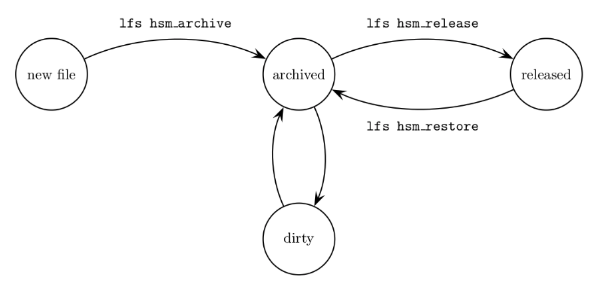
\includegraphics[width=\linewidth]{file.png}
    \caption{文件的状态的转换}\label{fig:region-image}
\end{figure}

\subsection{lustre的HSM架构设计}

lustre的HSM旨在提供一套多层存储的操作接口,并不提供接口的具体实现。在lustre的HSM中,文件的数据可以从lustre的OST中迁移到HSM存储中,但是文件的元数据信息,如文件名、用户ID、权限信息等将会一直保存在lustre的MDT中。当客户端打开一个已被release的文件或者主动执行restore操作时,lustre将自动从HSM中重新加载文件对应的数据。restore的整个过程如如下:

\begin{figure}[!htb]
    \centering
    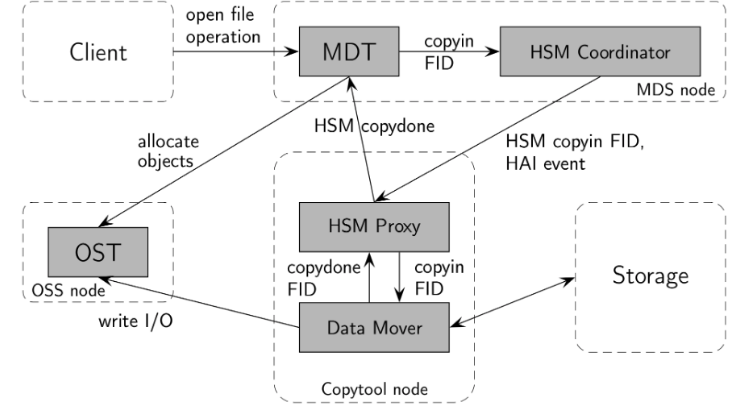
\includegraphics[width=\linewidth]{lustreHSM.png}
    \caption{HSM架构设计}\label{fig:region-image}
\end{figure}

客户端打开或者主动执行restore操作,该请求将首先被发送到相关的MDT服务中。MDT检测到文件的相应数据不在lustre中,将首先在OST中为该文件分配对应的存储空间,之后将文件的FID发送到HSM的CDT服务中。CDT服务解析该请求,并将该请求进一步封装发送到注册到该MDT中的合适的agent中。agent服务中产生对应的HSM事件,并从事件中解析到请求类型以及请求关联的FID。agent服务之后将请求进一步封装并发送到对应的Data Mover进程中。Data Mover服务具体的数据搬运工作,同时还可以进一步做一些数据的压缩、去重、加密等操作。在数据的搬运过程中,Data Mover可以向agent汇报数据搬运的进度,此时agent亦可将该进度汇报给CDT服务。数据搬运完成后Data Mover将向agent汇报数据搬运完成事件,之后agent将该事件进一步封装并汇报给MDT服务。MDT收到数据搬运完成的事件后将通知client文件打开成功。至此整个文件的restore完成。在此期间,客户端将一直处于阻塞状态。 

更一般的hsm请求控制流如下: 
\begin{lstlisting}[language={c++},numbers=left]
    1. 客户端调用llapi_hsm_request()创建hsm请求。 
    2. lustre client通过mdc_ioc_hsm_request()将该请求发送到mdt。 
    3. mdt创建相应的hsm请求日志llog,并唤醒cdt服务。 
    4. cdt服务被唤醒,从llog读取对应的日志内容,创建具体的HSM事件,并将事件发送到agent所在的客户端。 
    5. agent接收到hsm事件,并处理事件中封装的具体hsm请求
    6. agent可以随时调用llapi_hsm_action_progress()向CDT汇报数据搬运的进度。 
    7. 数据搬运完成后agent调用llapi_hsm_action_end()用于汇报mdt数据已搬运完成。 
\end{lstlisting}

\subsection{lustre MDT提供的HSM调节参数}

lustre的mdt参数项中包含一些关于hsm的参数。参数路径为/proc/fs/lustre/mdt/<fsname>/ 

% Please add the following required packages to your document preamble:
% \usepackage{graphicx}
\begin{table}[!htb]
    \centering
    \resizebox{\textwidth}{!}{%
    \begin{tabular}{|l|l|l|l|}
    \hline
    参数项                                   & 属性 & 释义                                                                                                                                                                      & 备注 \\ \hline
    hsm\_control                          & rw & \begin{tabular}[c]{@{}l@{}}控制cdt服务的启停,可选配置如下: \\ enabled:    开启cdt服务线程 \\ disabled:   暂停cdt一切服务 \\ shutdown: 关闭cdt服务,释放所有cdt资源 \\ purge:        清除所有的hsm请求\end{tabular} &    \\ \hline
    hsm/actions                           & r  &                                                                                                                                                                         &    \\ \hline
    hsm/active\_request\_timeout          & rw & 一个active请求执行的最大超时时间                                                                                                                                                     &    \\ \hline
    hsm/active\_requests                  & r  &                                                                                                                                                                         &    \\ \hline
    hsm/agents                            & r  & 查看当前已经注册的所有agent                                                                                                                                                        &    \\ \hline
    hsm/archive\_count                    & r  & 当前已经执行archive的统计计数                                                                                                                                                      &    \\ \hline
    hsm/default\_archive\_id              & rw & cdt 默认使用的archive ID                                                                                                                                                     &    \\ \hline
    hsm/grace\_delay                      & rw & 一个成功的或者失败的hsm请求被从请求列表中移除的最长时间                                                                                                                                           &    \\ \hline
    hsm/group\_request\_mask              & rw & 组访问权限相关                                                                                                                                                                 &    \\ \hline
    hsm/user\_request\_mask               & rw & 用户访问权限相关                                                                                                                                                                &    \\ \hline
    hsm/loop\_period                      & rw & hsm CDT扫描llog的周期                                                                                                                                                        &    \\ \hline
    hsm/max\_requests                     & rw & 每个mdt最大的active请求数                                                                                                                                                       &    \\ \hline
    hsm/policy                            & rw & \begin{tabular}[c]{@{}l@{}}hsm处理策略,\\ 有以下两种: NRA:No Retry Action, 如果restore失败,则不会再次执行 \\ NBR:Non Blocking Restore,如果访问一个已经被released的文件,将不会出发自动restore操作。\end{tabular}   &    \\ \hline
    hsm/remove\_archive\_on\_last\_unlink & rw & lustre文件中的数据被rm后是否发出hsm请求删除hsm存储中对应的数据。                                                                                                                                 &    \\ \hline
    hsm/remove\_count                     & r  &                                                                                                                                                                         &    \\ \hline
    hsm/restore\_count                    & r  &                                                                                                                                                                         &    \\ \hline
    \end{tabular}%
    }
    \caption{}
    \label{tab:my-table}
    \end{table}


\subsection{lustre的HSM接口}
lustre向外部导出C语言的API接口,主要的接口定义如下:
